% Stepwise augmentation scheme for the talk, adapted from docs/writeup/jan-blockscheme-v4.tex:
% same topology and notation; the setpoint generator is dropped (u_k is the motor-force input)
% and h_base is drawn without its u input. Words first: every block and signal is named in words,
% its thesis symbol second and smaller. \augstep selects how much is drawn:
%   1  physics model: f_base, the state register z^-1, the output map h_base
%   2  + neural network phi_aug, router S, f_aug into the Theta, X, Y updates; h_aug = 0
%   3  + learned states xbar, updated by g_aug; the network also reads xbar
%   4  + encoder psi: initial state from past inputs and outputs
% Parts introduced in the current step keep their role colour; earlier parts turn grey.
\documentclass[border=8pt]{standalone}
% Shared preamble of the TikZ slide figures. Role colours match style.py.
\usepackage[T1]{fontenc}
\usepackage[scaled]{helvet}
\renewcommand\familydefault{\sfdefault}
\usepackage{amsmath}
\usepackage{tikz}
\usetikzlibrary{arrows.meta,calc,decorations.pathmorphing,positioning}
\definecolor{cbase}{HTML}{D55E00}   % physics model
\definecolor{caug}{HTML}{0072B2}    % augmented model, no projection
\definecolor{cproj}{HTML}{009E73}   % augmented model with projection
\definecolor{cink}{HTML}{222222}
\definecolor{cmuted}{HTML}{6B6B6B}

\providecommand{\augstep}{4}
\colorlet{cold}{black!32}
\newcommand{\partof}[2]{%
  \ifnum#1>\augstep\relax\else
  \begin{scope}%
    \ifnum#1<\augstep\relax
      \colorlet{cbase}{cold}\colorlet{caug}{cold}\colorlet{cink}{cold}%
    \fi
    #2%
  \end{scope}%
  \fi}
\begin{document}
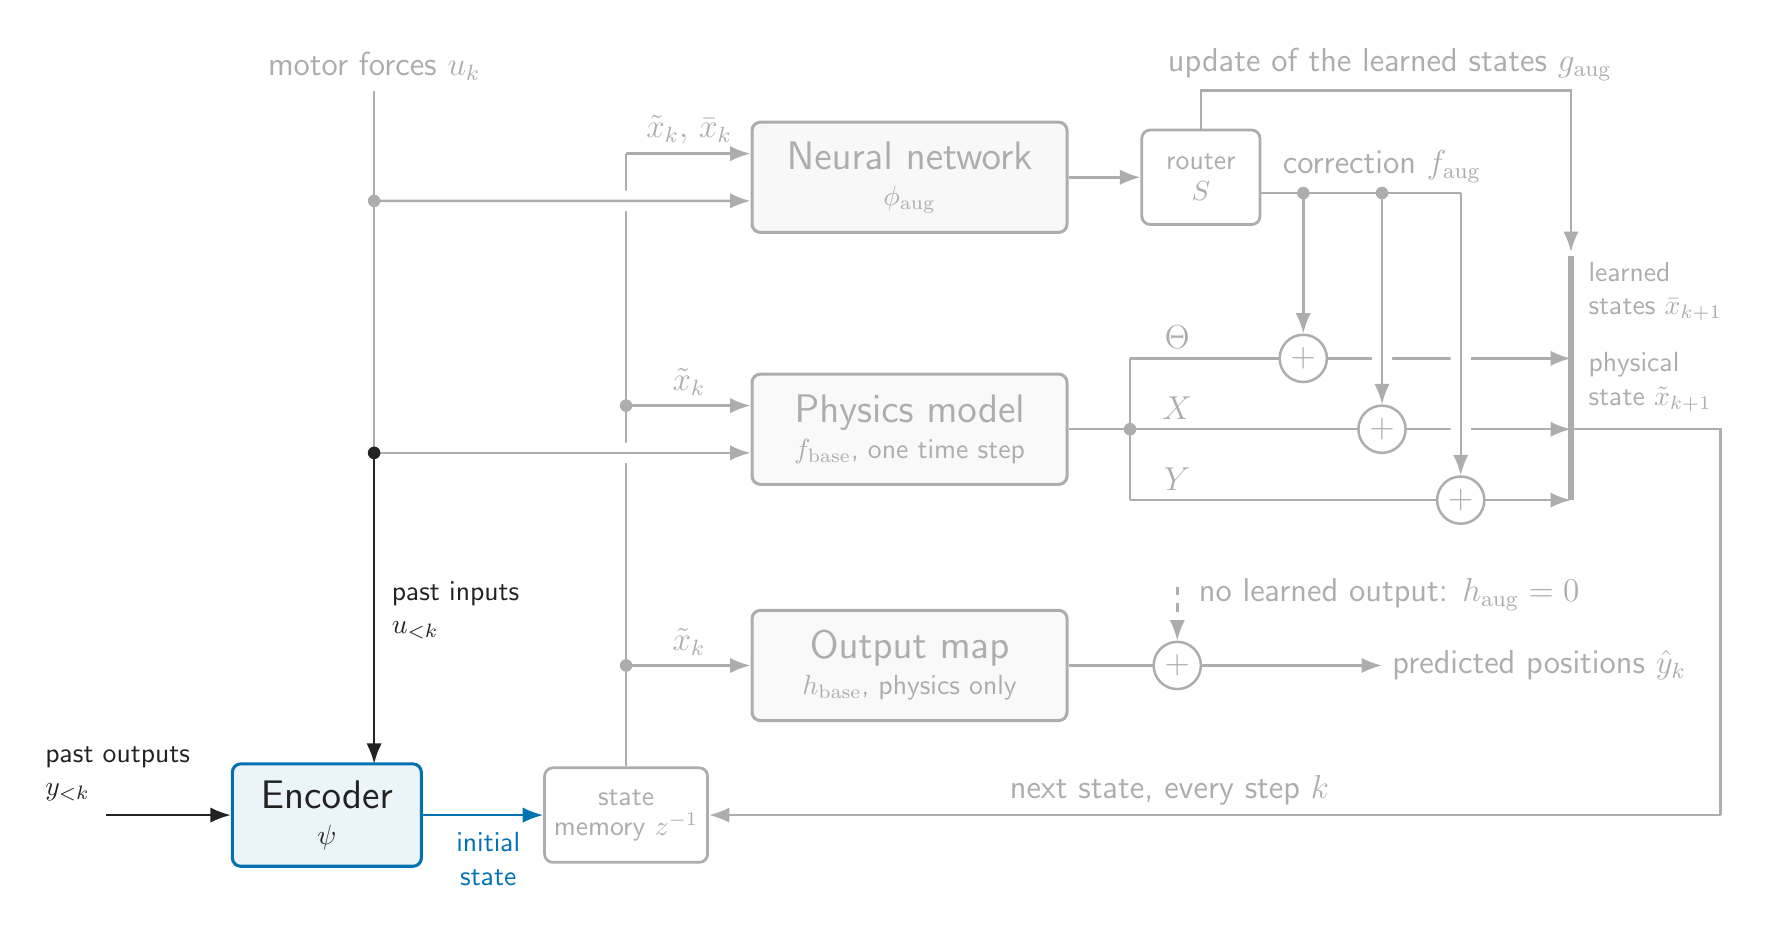
\begin{tikzpicture}[
    >={Latex[length=2.6mm]},
    sig/.style={->, line width=0.9pt, draw=cink},
    wire/.style={line width=0.9pt, draw=cink},
    blk/.style={draw, line width=1.1pt, rounded corners=3pt, align=center,
                minimum height=14mm, minimum width=40mm, text=cink},
    phys/.style={blk, draw=cbase, fill=cbase!7},
    ann/.style={blk, draw=caug, fill=caug!8},
    small/.style={draw=cink, line width=1pt, rounded corners=3pt, align=center, fill=white,
                  minimum width=18mm, minimum height=12mm, text=cink},
    sum/.style={draw=caug, line width=0.9pt, circle, fill=white, inner sep=0pt,
                minimum size=6mm, text=caug, font=\large},
    dot/.style={circle, fill=cink, inner sep=1.6pt},
    lbl/.style={font=\large, text=cink},
    note/.style={font=\normalsize, text=cink, align=left},
    gap/.style={fill=white, draw=none},
  ]
  % the same canvas in every step, so the four images overlay exactly on consecutive slides
  \path[use as bounding box] (-11.2,-6.1) rectangle (10.6,5.1);
  % == step 1: the physics model
  \partof{1}{
    \node[phys] (fb) at (0,0)
      {\Large Physics model\\[1pt]\normalsize $f_{\mathrm{base}}$, one time step};
    \node[phys] (hb) at (0,-3.0)
      {\Large Output map\\[1pt]\normalsize $h_{\mathrm{base}}$, physics only};
    \node[small] (dl) at (-3.6,-4.9)
      {\normalsize state\\[-1pt]\normalsize memory $z^{-1}$};
    % state bus and its taps
    \draw[wire] (dl.north) -- (-3.6,0.3);
    \draw[sig] (-3.6,0.3) -- ($(fb.west)+(0,0.3)$);
    \draw[sig] (-3.6,-3.0) -- (hb.west);
    \node[dot] at (-3.6,-3.0) {};
    \node[lbl, anchor=south] at (-2.8,0.3) {$\tilde x_k$};
    \node[lbl, anchor=south] at (-2.8,-3.0) {$\tilde x_k$};
    % input bus, crossing the state bus on a bridge
    \draw[wire] (-6.8,4.3) -- (-6.8,-0.3);
    \node[lbl, anchor=south] at (-6.8,4.3) {motor forces $u_k$};
    \fill[gap] (-3.6,-0.3) circle (1.3mm);
    \draw[sig] (-6.8,-0.3) -- ($(fb.west)+(0,-0.3)$);
    % the three physical channels into the next-state bar
    \draw[sig] (fb.east) -- (8.4,0);
    \draw[wire] (2.8,-0.9) -- (2.8,0.9);
    \node[dot] at (2.8,0) {};
    \draw[sig] (2.8,0.9) -- (8.4,0.9);
    \draw[sig] (2.8,-0.9) -- (8.4,-0.9);
    \node[lbl, anchor=south] at (3.4,0.9) {$\Theta$};
    \node[lbl, anchor=south] at (3.4,0) {$X$};
    \node[lbl, anchor=south] at (3.4,-0.9) {$Y$};
    \draw[line width=2.2pt, draw=cink] (8.4,-0.9) -- (8.4,0.9);
    \node[note, anchor=south west] at (8.5,0.1) {physical\\state $\tilde x_{k+1}$};
    % next state back to the state memory
    \draw[wire] (8.4,0) -- (10.3,0) -- (10.3,-4.9);
    \draw[sig] (10.3,-4.9) -- (dl.east);
    \node[lbl, anchor=south] at (3.3,-4.9) {next state, every step $k$};
    % output
    \draw[sig] (hb.east) -- (6.0,-3.0)
      node[lbl, anchor=west] {predicted positions $\hat y_k$};
  }
  % == step 2: the neural network and its routing
  \partof{2}{
    \node[ann] (an) at (0,3.2)
      {\Large Neural network\\[1pt]\normalsize $\phi_{\mathrm{aug}}$};
    \node[small, draw=caug, text=caug, minimum width=15mm] (S) at (3.7,3.2)
      {\normalsize router\\[-1pt]\normalsize $S$};
    % state bus extended to the network
    \draw[wire] (-3.6,0.3) -- (-3.6,3.5);
    \node[dot] at (-3.6,0.3) {};
    \draw[sig] (-3.6,3.5) -- ($(an.west)+(0,0.3)$);
    \ifnum\augstep<3\relax
      \node[lbl, anchor=south] at (-2.8,3.5) {$\tilde x_k$};
    \fi
    \fill[gap] (-3.6,2.9) circle (1.3mm);
    \draw[sig] (-6.8,2.9) -- ($(an.west)+(0,-0.3)$);
    \node[dot] at (-6.8,2.9) {};
    % network output routed into Theta, X and Y
    \draw[sig, draw=caug] (an.east) -- (S.west);
    \draw[line width=0.9pt, draw=caug] ($(S.east)+(0,-0.2)$) -- (7.0,3.0);
    \node[lbl, text=caug, anchor=south] at (6.0,3.0) {correction $f_{\mathrm{aug}}$};
    \fill[gap] (6.0,0.9) circle (1.3mm);
    \fill[gap] (7.0,0.9) circle (1.3mm);
    \fill[gap] (7.0,0) circle (1.3mm);
    \node[sum] (sT) at (5.0,0.9) {$+$};
    \node[sum] (sX) at (6.0,0) {$+$};
    \node[sum] (sY) at (7.0,-0.9) {$+$};
    \draw[sig, draw=caug] (5.0,3.0) -- (sT.north);
    \draw[sig, draw=caug] (6.0,3.0) -- (sX.north);
    \draw[sig, draw=caug] (7.0,3.0) -- (sY.north);
    \node[dot, fill=caug] at (5.0,3.0) {};
    \node[dot, fill=caug] at (6.0,3.0) {};
    % the output map stays physical
    \node[sum] (sO) at (3.4,-3.0) {$+$};
    \draw[->, line width=0.9pt, draw=caug, dashed] (3.4,-2.0) -- (sO.north);
    \node[lbl, text=caug, anchor=west] at (3.55,-2.1)
      {no learned output: $h_{\mathrm{aug}}=0$};
  }
  % == step 3: the learned states
  \partof{3}{
    \node[lbl, text=caug, anchor=south] at (-2.8,3.5) {$\tilde x_k,\,\bar x_k$};
    \draw[line width=2.2pt, draw=caug] (8.4,0.9) -- (8.4,2.2);
    \draw[sig, draw=caug] (S.north) -- (3.7,4.3) -- (8.4,4.3) -- (8.4,2.25);
    \node[lbl, text=caug, anchor=south] at (6.1,4.3)
      {update of the learned states $g_{\mathrm{aug}}$};
    \node[note, text=caug, anchor=south west] at (8.5,1.25) {learned\\states $\bar x_{k+1}$};
  }
  % == step 4: the encoder sets the initial state
  \partof{4}{
    \node[ann, minimum width=24mm, minimum height=13mm] (en) at (-7.4,-4.9)
      {\Large Encoder\\[1pt]\normalsize $\psi$};
    \draw[sig] (-6.8,-0.3) -- (-6.8,-4.25);
    \node[dot] at (-6.8,-0.3) {};
    \node[note, anchor=west] at (-6.7,-2.3) {past inputs\\$u_{<k}$};
    \draw[sig] (-10.2,-4.9) -- (en.west);
    \node[note, anchor=south west] at (-11.1,-4.85) {past outputs\\$y_{<k}$};
    \draw[sig, draw=caug] (en.east) -- (dl.west);
    \node[font=\normalsize, text=caug, align=center, anchor=north] at (-5.35,-5.0)
      {initial\\state};
  }
\end{tikzpicture}
\end{document}
